\section{Literature Review}
\subsection{Preamble}
There is a rich variety of research available in the field of applying machine learning techniques to stock market trading. The earliest originate in the late 90's and cover a range of very specific niches within the field, from portfolio management and stock price forecasting, to establishing trading rules for automatic stock screeners. \newline

To achieve these aims, an assortment of different machine learning techniques are utilised. Notably, the style of machine learning changes over time, with Genetic Algorithms being more popular in the early 00's and Neural Networks being the current go-to method.

\subsection{Financial Forecasting Using GAs \cite{mahfoudMani}}
This first paper outlines ``a new system that utilizes genetic algorithms...to predict the future performances of individual stocks''.

\subsubsection{Genetic Algorithms and Chromosomes}

It begins by outlining the basic terminology within Machine Learning and Genetic Algorithms, particularly the concepts of Mutation and Crossover within the field of GAs. A key term defined early on is ``genetic material'' (nowadays commonly referred to as the Chromosome or the Genotype). The Chromosome (Genotype) is a set of parameters which define a proposed solution (Phenotype). In layman's terms, the solution is a specific realisation of the chromosome. \newline

The author makes a key distinction here, saying that the algorithm ``implicitly processes...the genetic material (chromosomes)...and not individual solutions''. This is an important separation of concepts; the algorithm does not transform existing solutions into new solutions, it transforms the set of possible solutions into a new set of possible solutions, which is ``better'' in some definable fashion. \newline

The paper then gives a specific example saying ``...a GA may discover that one variable, such as price-to-earnings ratio, is a better indicator of future return than another, such as past return''. This is the core feature of genetic algorithms that enable them to search their domain more efficiently; they can bias in favour of the better ``dimension'', the more important rule in the chromosome.

\subsubsection{Michigan Vs Pittsburgh}

There are two approaches to how populations work within genetic algorithms. Either the population in its entirety forms one chromosome with each member being one part of that chromosome (Michigan approach), or every member is a chromosome and the population is a pool of viable chromosomes (Pittsburgh approach). This study in particular uses the Michigan approach, whilst I intend to use Pittsburgh. \newline

The reason given in the study for this choice is that Pittsburgh constitutes a ``large handicap on a GA-based learner'', in terms of time efficiency. However, this is a paper from 20 years ago and concerns of learning speed due to large data size are far less relevant in the modern day. The vast majority of modern genetic algorithms use the Pittsburgh approach, as it is conceptually closer to the idea of evolution that the algorithm endeavours to recreate.

\subsubsection{Niching}

A short discussion on the benefits of niching comes next. Niching is the process of only allowing chromosomes to compete with each other if they are sufficiently similar. This can allow a good deal of variation to be present within the population, as the algorithm can optimise multiple potential chromosomes at once, each chromosome being wildly different. \newline

The author goes on to specify that this is a useful construct within the field of financial prediction as ``different rules within a single population can perform forecasting under different market environments''.

\subsubsection{The Experiments}

The core of the study consists of two experiments, both effectively the same but the second at a larger scale; presumably this was done in case the second experiment wasn't successful so the authors would at least have something to report. Due to the similarity between these experiments, I am going to ignore the first one. \newline

In both experiments the authors genetic algorithm is compared to a neural network performing the same task. The task here is the classification of stocks into three categories: buy, sell, and no opinion. The algorithm is set up such that ``both GA and NN forecasts are made at the end of the week for three consecutive weeks. Each weekend, forecasts are made for over 1600 stocks. Twelve weeks after each forecast, the forecasts are compared with actual 12-week relative returns.'' \newline

The GA and NN predict both the ``magnitude and direction of the return of each stock, relative to the market''. Extra statistics are then calculated such as the average returns of the positive and negative forecasts, as well as a measure of the spread between these two averages, with high spread implying a better set of predictions.

\subsubsection{The Results}

The GAs outperformed the NNs overall with a larger spread (2.16\% versus 1.4\%) and better mean relative return performance over the top two quintiles (typically only stocks in the top two quintiles of this statistic are traded). \newline

The author goes on to reference a prior paper by Mahfoud \& Mani from 1995, suggesting that ``an approach that utilizes both GA and NN forecasts is superior to utilizing the better of the two algorithms, in isolation''. The author demonstrates that this hypothesis was correct in this experiment, with ``an average relative return of 6.61\% in the top quintile of the positive combined forecasts. This is a 21\% improvement over the GAs alone, and a 50\% improvement over the NNs alone.''

\subsubsection{GA versus NN}

The final discussion the author presents is whether GAs or NNs are better for this style of application. The author does not conclude that either method is superior to the other, referring to both methods as ``promising''. The author continues, suggesting that this promise is ``due to their ability to learn nonlinear relationships ... (that) are typically not apparent to the average market participant''. In other words, the algorithms can spot trends that a human observer (or a less sophisticated computer method) could not reliably notice. \newline

The author attributes the better performance of the GAs to their ability to abstain from predicting (which was done 27\% of the time), whereas the neural network was forced to always predict. This is quite a significant functional difference, which throws the overall result into doubt; the comparison between the two systems is hardly fair if only one of them enjoys more advanced features. \newline

The last comment that I wish to highlight is that GAs have the ability to output ``comprehensible rules''. Unlike black box methods like NNs, the GAs output can be easily designed to be human readable. This allows the output of the GA to be easily examined, and for it to be compared - immediately and directly - with human designed methods.

\subsection{Using GAs to find Technical Trading rules \cite{allenKarjalainen}}
This second study experiments with a genetic algorithm ``to learn technical trading rules for the S\&P 500 index using daily prices from 1928 to 1995.'' This is much closer to what I am trying to achieve than the first paper.

\subsubsection{Introduction}
The paper begins by stating its purpose: ``to demonstrate how they (Genetic Algorithms) can be used to find technical trading rules.'' It continues with a presentation of past literature, stating that ``such rules do not make money''. \newline

A number of studies are referenced, including Fama (1970) which ``dismiss(ed) technical analysis as a futile undertaking'' \cite{fama70}. Brock et al. (1992) was slightly more hopeful, showing that ``in the absence of transaction costs ... these rules identify periods to be in the market when returns are high and volatility is low (and vice versa)'' \cite{brock92}.

\subsubsection{Genetic Algorithms Overview}
The second chapter presents an overview of the basics of Evolutionary Algorithms as well as Genetic Programming. I am motivated to skip this section as I intend to provide my own summary of the relevant concepts within Evolutionary Algorithms in a later chapter, but also, there are several statements from this chapter which are no longer accurate. \newline

For example, the author states that ``solution candidates are represented as character strings from a given (often binary) alphabet.'' Whilst this is still a valid method to represent solution candidates, advances in the complexity of computers have allowed for more elaborate representations than simple bit strings. \newline

There is a related comment later in the section stating that evolutionary algorithms ``embody very little problem-specific knowledge''. This is incorrect; evolutionary algorithms can be customised in a variety of ways to their problem domain, most specifically with regards to the fitness function (which the author themselves concedes in chapter 2.1 paragraph 2) and problem representation. A custom representation then demands at least custom crossover and mutation functions, and perhaps even requiring a custom selection function as well.

\subsubsection{Representing Trading Rules}
After introducing Genetic Programming in the last chapter, the authors go into detail as to how they will represent their trading rules as genetic programs. \newline

The rules are constructed as trees, from a variety of mathematical and logical operators. Each tree corresponds to a boolean expression which at any point in time is either true or false. The authors provide two simple example rules:
\begin{figure}[h]
    \centering
    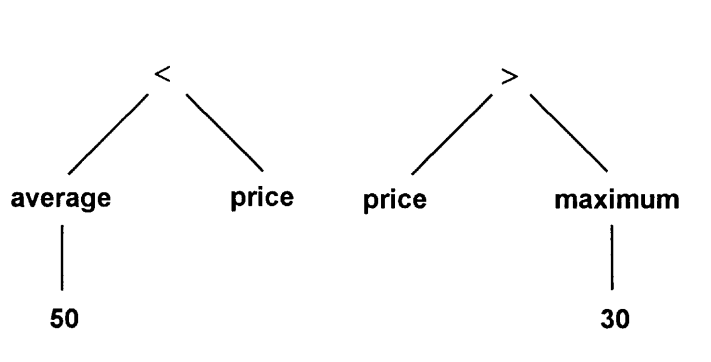
\includegraphics[width=0.5\textwidth]{images/averageAndMax.png}
\end{figure}

The left tree represents a rule which evaluates true if the current stock price is greater than a 50 day moving average of the stock price, and the right represents a rule which evaluates true if the current stock price is greater than the 30 day maximum stock price. \newline 

The author continues by defining the necessary crossover operator for this tree representation, as well as an appropriate fitness function.

\subsubsection{Overfitting}
After discussing representation, the author stresses the need to address the ``possibility of overfitting the training data''. Overfitting can occur in machine learning algorithms for a variety of reasons, but most stem from having a lack of data:
\begin{itemize}
    \item Small Data Set - The algorithm can only detect trends over the data it has. If the data set is small, the algorithm has less chance to detect common trends.
    \item Training Data Reuse - Small data sets may necessitate that the algorithm be repeatedly trained over the same data. Unless precautions are taken, this may result in the algorithm learning the data set as opposed to learning its trends.
    \item Evaluating on Training Data - If the algorithm is evaluated on data that it has already seen (data that it was trained on), then it is likely to give inaccurate results.
\end{itemize}

The author proposes a series of options to tackle this overfitting, including ``reserving
a part of the data as a validation set on which to test the predictions, increasing
the amount of training data, penalizing for model complexity, and minimizing
the amount of information needed to describe both the model and the data''. The author opts to implement the first of these suggestions.

\subsubsection{Results}
The results of the algorithm are not particularly encouraging. Running their algorithm 100 times, the authors generate 89 trading rules. The excess return of these rules is predominantly negative (meaning that the rules did not outperform the strategy of buying and holding), and the trading frequency is low with 3.8 trades per year on average. The results are marginally better when transaction fees are lowered, and marginally worse when they are increased. \newline

The author summarises, saying ``the out-of-sample test results indicate that the trading rules do not earn consistent excess returns after transaction costs. Nevertheless, they appear to have some ability to forecast daily returns.'' \newline

They end with some criticisms on their algorithm, specifically that their ``parameters are not necessarily optimal'', as well as stating that ``it would be interesting to apply a similar technique to learn fundamental trading rules,'' which is what I intend to do with my algorithm.